\chapter{Conexión local con BD externa}

Aunque la base de datos de Eunomia permite satisfacer las necesidades ''demo'' de la herramienta, en la mayoría de las ocasiones el objetivo final de la implementación de ATLAS es realizar un estudio o investigación específica sobre una base de datos externa, específica del usuario o la organización que incopora la herramienta de análisis. 

Por tanto, es de gran interés presentar cómo establecer una conexión adicional entre ATLAS Broadsea y una base de datos personalizada o propia, más allá de la demo que viene inicializada con el contenedor.

\section{Obtener otras BD}

- synthea
- synpuf

\section{Requisitos previos} \label{cap:04RequisitosPrevios}

- BD en forma CDM
- Ejemplo con synthea: en el mismo servidor,  no hay equema temp, y tampoco vocab porque se va a utilizar el por defecto

\section{Deployment}

La conexión con la base de datos externa se puede realizar de dos formas distintas: (a) a través de el administrador de la base de datos o (b) activando un protocolo de seguridad de ATLAS. 

En este manual se presentan ambas opciones aunque solo se seguirá en profundidad el protocolo de conexión mediante el administrador de la base de datos (a), ya que es la opción más sencilla y que los propios desarrolladores recomiendan para una implementación rápida \cite{forumAddMSDB}. Por otra parte, por la naturaleza del entorno de instalación al que se enfoca este manual (descrita en \ref{cap:Introduccion al manual}), no es de interés activar el protocolo de seguridad de ATLAS, que debería ser la opción preferente para el despligue de la herramienta en organizaciones donde haya una diferenciación entre usuarios administradores con privilegios y usuarios sin privilegios. Sin embargo, este caso no aplica puesto que la implementación se realiza para un grupo de investigadores en la que todos tienen los mismos privilegios de acceso.

\subsection{A través del administrador de la base de datos}

La conexión con la base de datos a través del administrador de la base de datos, en este caso pgAdmin, es bastante sencilla, basta con configurar los parámetros correspondientes en el esquema \code{webapi} de la base de datos de Broadsea. Esta implementación se describe de forma muy completa en la documentación correspondiente al repositorio de github de CDM Configuration \cite{githubCDMConfiguration} y en los foros \cite{forumAddMSDB}\cite{forumBroadQuickStart}.

\begin{enumerate}
    \item En primer lugar, se debe añadir la nueva fuente en la tabla \code{sources} del esquema \code{webapi}. De este modo se registra la nueva fuente y el string jdbc que apunta hacia ella permitiendo la conexión. Para ello se puede utilizar la siguiente query genérica \cite{githubCDMConfiguration}:

\begin{lstlisting}[language=sql]
INSERT INTO webapi.source (source_id, source_name, source_key, source_connection, source_dialect) 
SELECT nextval('webapi.source_sequence'), 'My Cdm', 'MY_CDM', ' jdbc:postgresql://server:5432/cdm?user={user}&password={password}', 'postgresql';
\end{lstlisting}

    Donde:
    \begin{itemize}
        \item \code{source\_id}: Es el identificador de la fuente. Se asigna por defecto.
        \item \code{source\_name}: Es el nombre personalizado de la fuente.
        \item \code{source\_key}: Es la clave que utilizarán otras tablas para referirse a la fuente.
        \item \code{source\_connection}: Es el string de conexión jdbc, que debe seguir la estructura por defecto que se suigiere en la query. Si la
        \item \code{source\_dialect}: El dialecto que utiliza la base de datos. Por defecto sería postgresql.
    \end{itemize}

    Para la realización de esta implementación de ejemplo se ha seguido el ejemplo de synthea (descrito en \ref{cap:04RequisitosPrevios}), que aplica la siguiente query:

\begin{lstlisting}[language=sql]
INSERT INTO webapi.source (source_id, source_name, source_key, source_connection, source_dialect) 
SELECT nextval('webapi.source_sequence'), 'synthea1k', 'SYNTHEA1K', ' jdbc:postgresql://broadsea-atlasdb:5432/synthea1k?user=postgres&password=mypass', 'postgresql';
\end{lstlisting}

    Esto obtiene como resultado global:

\begin{figure}[H]
    \centering
    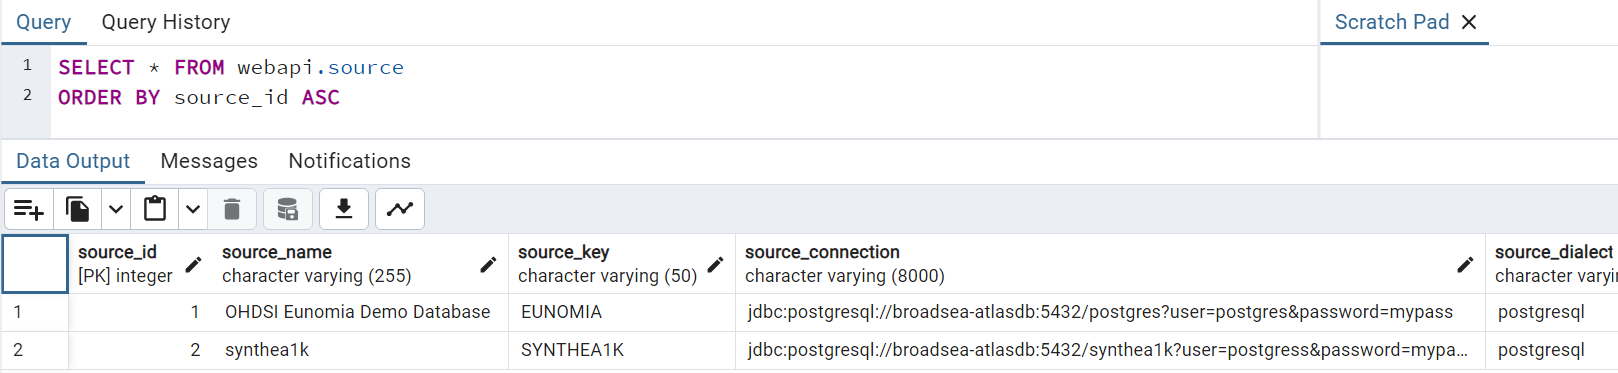
\includegraphics[width=0.90\textwidth]{figures/querySource.png}
    \caption{Captura de pantalla de las fuentes registradas en la tabla \code{sources}.}
    \label{fig:querySource}
\end{figure}
    

    \item En segundo lugar, y por último, se debe registrar cada esquema que utiliza la nueva fuente en la tabla \code{source\_daimon} del esquema \code{webapi}. Para ello se pueden utilizar las siguientes queries genéricas \cite{githubCDMConfiguration}:

\begin{lstlisting}[language=sql]
INSERT INTO webapi.source_daimon (source_daimon_id, source_id, daimon_type, table_qualifier, priority) 
SELECT nextval('webapi.source_daimon_sequence'), source_id, 0, 'cdm', 0
FROM webapi.source
WHERE source_key = 'MY_CDM';

INSERT INTO webapi.source_daimon (source_daimon_id, source_id, daimon_type, table_qualifier, priority) 
SELECT nextval('webapi.source_daimon_sequence'), source_id, 1, 'vocab', 1
FROM webapi.source
WHERE source_key = 'MY_CDM';

INSERT INTO webapi.source_daimon (source_daimon_id, source_id, daimon_type, table_qualifier, priority) 
SELECT nextval('webapi.source_daimon_sequence'), source_id, 2, 'results', 1
FROM webapi.source
WHERE source_key = 'MY_CDM';

INSERT INTO webapi.source_daimon (source_daimon_id, source_id, daimon_type, table_qualifier, priority) 
SELECT nextval('webapi.source_daimon_sequence'), source_id, 5, 'temp', 0
FROM webapi.source
WHERE source_key = 'MY_CDM';
\end{lstlisting}

    Donde:
    \begin{itemize}
        \item \code{source\_daimon\_id}: Es el identificador del daimon. Se asigna por defecto.
        \item \code{source\_id}: Es el identificador de la nueva fuente, según el valor obtenido al registrar la fuente en la tabla \code{sources}.
        \item \code{daimon\_type}: Es el identificador que designa tipo de daimon que se está registrando, es decir, el tipo de esquema. Este identificador puede ser ''0'' para el esquema del \code{cdm}, ''1'' para el \code{vocab}, ''2'' para \code{results} y, opcionalmente, ''5'' para \code{temp}.
        \item \code{table\_qualifier}: Es el nombre concreto del esquema al que se está apuntando.
        \item \code{priority}: \color{red}{valor entero mayor o menor que uno para ordenar}.
    \end{itemize}

    Para la realización de esta implementación de ejemplo se ha seguido el ejemplo de synthea (\ref{cap:04RequisitosPrevios}), que aplica las siguiente queries:

\begin{lstlisting}[language=sql]
INSERT INTO webapi.source_daimon (source_daimon_id, source_id, daimon_type, table_qualifier, priority) 
SELECT nextval('webapi.source_daimon_sequence'), source_id, 0, 'synthea', 0
FROM webapi.source
WHERE source_key = 'SYNTHEA1K';

INSERT INTO webapi.source_daimon (source_daimon_id, source_id, daimon_type, table_qualifier, priority) 
SELECT nextval('webapi.source_daimon_sequence'), 2, 1, 'cdm', 1
FROM webapi.source
WHERE source_key = 'SYNTHEA1K';

INSERT INTO webapi.source_daimon (source_daimon_id, source_id, daimon_type, table_qualifier, priority) 
SELECT nextval('webapi.source_daimon_sequence'), 2, 2, 'cdm_results', 0
FROM webapi.source
WHERE source_key = 'SYNTHEA1K';
\end{lstlisting}

    Esto se obtiene como resultado global:

\begin{figure}[H]
    \centering
    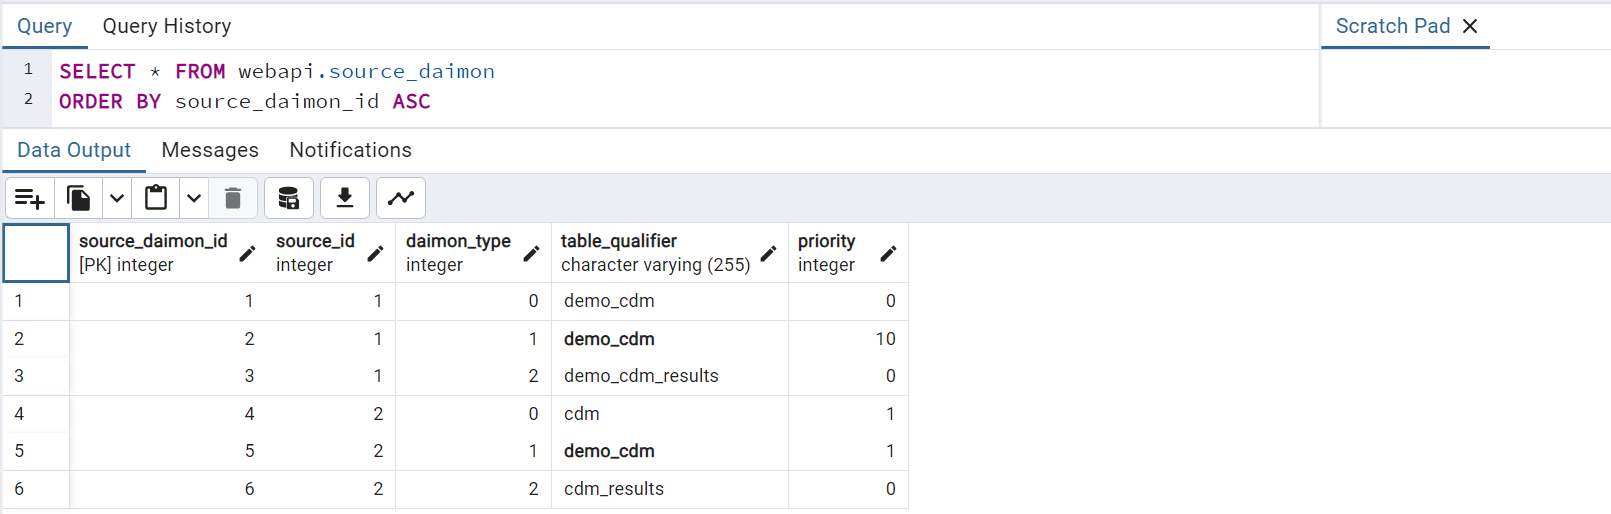
\includegraphics[width=0.90\textwidth]{figures/queryDaimon.png}
    \caption{Captura de pantalla de los daimon registrados en la tabla \code{source\_daimon}.}
    \label{fig:queryDaimon}
\end{figure}

    Observe que si se agrupase por \code{source\_id} hay dos fuentes distintas: (1) la fuente demo que viene preoconfigurada con Broadsea y (2) la fuente que se acaba de registrar.

\end{enumerate}

Así de sencillamente ya estaría registrada la nueva fuente, y establecida la conexión con la misma a través de la webAPI de Broadsea.


\subsection{A través del protocolo de seguridad de ATLAS}

- No procede porque da muchos erroes
- Diferencia entre usuarios (mirar el .env file)
- Ni siquiera lo recomiendan aqui: https://forums.ohdsi.org/t/adding-a-new-ms-sql-cdm-database-to-atlas-using-broadsea/19404/2 

- Entiendo que es cuando se va a ejecutar en un entonro empresarial que verdaderamente necesite distinguir usuarios que pueden añadir data sources y usuariosq ue solo pueden manipular la herramienta. En este caso, como es un departamento de investigación todos los investigadores tienen los mismos privilegios, es una tonteria establecer la seguridad. Nada mñas que es una posible fuente de problemas.

\section{Comprobación de conexión correcta}

- mirar 127.0.01/sources


\section{Solución de posibles problemas}

- Faltan esquemas no aparece
- Valores mla introducidos
